\pdfinfoomitdate=1
\pdftrailerid{}
\pdfsuppressptexinfo=15
\documentclass[9pt]{article}
\usepackage[margin=0.62in]{geometry}
\usepackage{amsmath,amssymb,amsthm,booktabs,graphicx,microtype,caption}
\usepackage[T1]{fontenc}
\newtheorem{proposition}{Proposition}
\setlength{\parindent}{0pt}
\setlength{\parskip}{0.35em}
\title{\vspace{-2.2em}DRPO Pipeline v2.3 Core: Faithful Outline-to-Blueprint Slice}
\author{Anonymous review artifact}
\date{}
\begin{document}
\maketitle
\vspace{-2.0em}
\textbf{Scope.}
This two-page artifact validates the manuscript pipeline, not a new experiment.
It preserves the approved paragraph identities \texttt{METHOD-P03} and
\texttt{EXP-P04} without merge, split, rename, or reorder. It uses the
long-run-validated C-U1-E3-ADAM-RERUN compact repository evidence.
C-U1 evaluates same-distribution held-out-context generalization, and task,
boundary, and NaN/Inf events remain separate.

\section*{Proposition 2: Vanishing Weighted Far-Field Gradient}
The exponential envelope is selected for a precise tail property rather than an assumed utility-decay law. Under the finite-order score-growth condition in Proposition 2, multiplying the unweighted score-times-advantage contribution by exp(-lambda r) drives the weighted far-field term to zero as policy-relative remoteness grows. This is a method-level tail guarantee: it neither ranks all tapers nor claims that sample utility itself decays exponentially.
\setcounter{proposition}{1}
\begin{proposition}[Vanishing weighted far-field gradient]
\label{prop:far-field}
Let $r\geq 0$ be policy-relative remoteness and suppose the unweighted
score-times-advantage contribution satisfies
$\lVert g(r)\rVert\leq C(1+r)^k$ for finite constants $C>0$ and $k\geq 0$.
For any $\lambda>0$, define $\widetilde g(r)=e^{-\lambda r}g(r)$.
Then $\lVert\widetilde g(r)\rVert\to 0$ as $r\to\infty$.
\end{proposition}

\begin{proof}
The assumption gives
\[
  \lVert\widetilde g(r)\rVert
  \leq C(1+r)^k e^{-\lambda r}.
\]
For integer $m>k$, the exponential series implies
$e^{\lambda r}\geq (\lambda r)^m/m!$ for $r>0$. Hence
\[
  (1+r)^k e^{-\lambda r}
  \leq \frac{m!(1+r)^k}{(\lambda r)^m},
\]
and the right-hand side converges to zero because $m>k$. The squeeze theorem
proves the result. The proposition controls the weighted gradient tail; it
makes no assumption that sample utility decays exponentially.
\end{proof}


\textbf{Claim boundary.}
The proposition controls the weighted gradient tail under finite-order score
growth. It does not assume exponential utility decay and does not establish a
universal ranking among taper families.

\clearpage
\section*{RQ2b: Targeted Causal Transmission}
\vspace{-0.5em}
\begin{center}
\begin{minipage}[t]{0.49\textwidth}
\centering
\captionsetup{type=table,font=footnotesize,skip=3pt}
\captionof{table}{Terminal outcomes. Task, support-boundary, and NaN/Inf events are separate.}
\label{tab:cu1-e3}
\scriptsize
\resizebox{\linewidth}{!}{\begin{tabular}{@{}lrrrr@{}}
\toprule
Method & Fixed reward (95\% CI) & Task & Support & NaN/Inf \\
\midrule
Baseline & 2.22e-06 [2.10e-06, 2.35e-06] & 20/20 & 20/20 & 0/20 \\
Near-zero & 2.18e-06 [2.05e-06, 2.30e-06] & 20/20 & 20/20 & 0/20 \\
Far-zero & 0.739 [0.739, 0.740] & 0/20 & 0/20 & 0/20 \\
Far-cap & 0.733 [0.733, 0.734] & 0/20 & 0/20 & 0/20 \\
Global-scale & 0.599 [0.599, 0.599] & 0/20 & 0/20 & 0/20 \\
Far-to-near & 0.875 [0.875, 0.876] & 0/20 & -- & 0/20 \\
\bottomrule
\end{tabular}
}
\end{minipage}\hfill
\begin{minipage}[t]{0.49\textwidth}
\centering
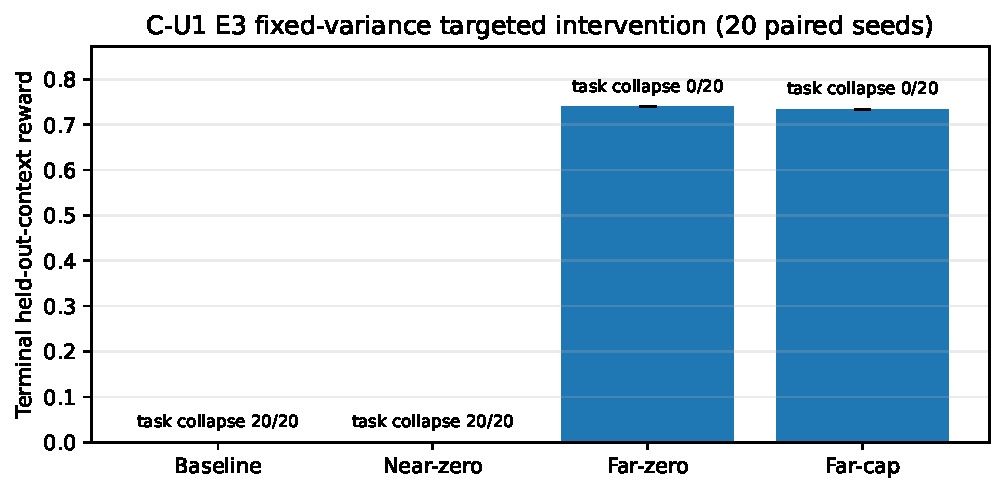
\includegraphics[width=\linewidth]{cu1_e3_fixed_reward.pdf}
\captionsetup{type=figure,font=footnotesize,skip=3pt}
\captionof{figure}{Fixed-variance terminal reward with 95\% CIs; labels show task-collapse counts.}
\label{fig:cu1-e3}
\end{minipage}
\end{center}
\vspace{-0.4em}

We test the registered transmission path with four matched interventions over 20 paired held-out seeds and report task, boundary, and numerical events separately. In the fixed-variance branch, Baseline and Near-zero finish at rewards 2.22e-06 and 2.18e-06 and undergo task-performance collapse in 20/20 and 20/20 seeds. Far-zero instead reaches 0.739 [0.739, 0.740], and Far-cap reaches 0.733 [0.733, 0.734], with no task collapse. The registered budget controls also remain non-collapsed: Global-scale reaches 0.599, while transferring the far budget to the near component reaches 0.875; these controls diagnose the pathway rather than establish a universal method ranking. The learnable-variance branch reaches the support/variance-contraction boundary in 20/20 Baseline and 20/20 Near-zero seeds, with mean onsets at steps 72.9 and 73.1, whereas Far-zero and Far-cap record 0/20 and 0/20 such events. All four methods retain finite parameters and record 0/20 NaN/Inf failures. Within this controlled same-distribution held-out-context setting, the near-removal non-rescue, far removal/capping rescue, and fixed-budget controls identify the far-field component as the dominant causal transmission path without extending that conclusion to universal off-policy behavior.

\section*{Pipeline audit}
The approved outline is compiled into a 39-node AST. Every node receives an
explicit enabled or disabled status; the two enabled nodes map one-to-one into
the blueprint and prose. Every empirical number is rendered from
\texttt{research\_snapshot.json}. Missing evidence fails closed rather than
creating a placeholder result.

\end{document}
